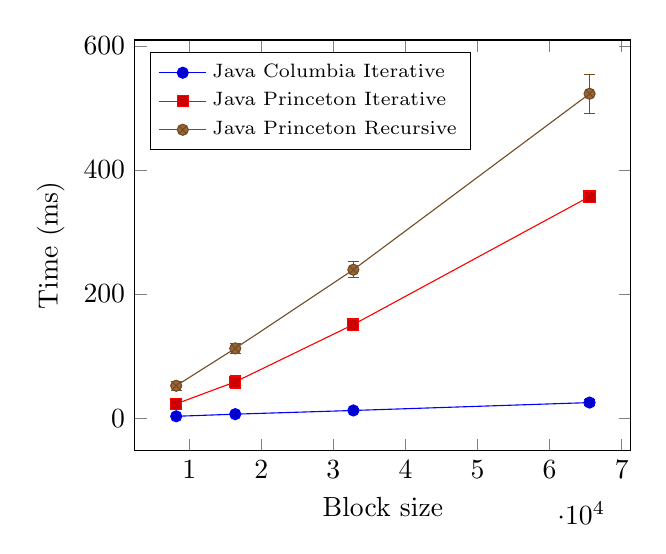
\begin{tikzpicture}
\begin{axis}[xlabel={Block size},ylabel={Time (ms)},width=0.65\linewidth,legend pos=north west,legend cell align=left,legend style={font=\scriptsize}]
\addplot+[error bars/.cd, y dir=both,y explicit] coordinates {
(8192, 2.8726) +- (0.3247, 0.3247)
(16384, 6.3214) +- (1.0542, 1.0542)
(32768, 12.2634) +- (2.9076, 2.9076)
(65536, 24.9874) +- (4.6266, 4.6266)
};
\addplot+[error bars/.cd, y dir=both,y explicit] coordinates {
(8192, 22.9609) +- (5.6248, 5.6248)
(16384, 58.3825) +- (9.9410, 9.9410)
(32768, 150.7299) +- (5.5432, 5.5432)
(65536, 356.9871) +- (8.0942, 8.0942)
};
\addplot+[error bars/.cd, y dir=both,y explicit] coordinates {
(8192, 52.0853) +- (7.1292, 7.1292)
(16384, 112.3024) +- (8.1890, 8.1890)
(32768, 239.0777) +- (12.8962, 12.8962)
(65536, 522.7409) +- (31.4586, 31.4586)
};
\legend{Java Columbia Iterative , Java Princeton Iterative , Java Princeton Recursive}
\end{axis}
\end{tikzpicture}
